% Created 2017-04-18 Tue 11:09
% Intended LaTeX compiler: pdflatex
\documentclass[a4paper,11pt]{article}
\usepackage[utf8]{inputenc}
\usepackage[T1]{fontenc}
\usepackage{graphicx}
\usepackage{grffile}
\usepackage{longtable}
\usepackage{wrapfig}
\usepackage{rotating}
\usepackage[normalem]{ulem}
\usepackage{amsmath}
\usepackage{textcomp}
\usepackage{amssymb}
\usepackage{capt-of}
\usepackage{hyperref}
\usepackage[margin=1in]{geometry}
\usepackage{setspace}
\onehalfspacing
\usepackage{parskip}
\usepackage{mathtools}
\usepackage{hyperref}
\hypersetup{colorlinks,citecolor=black,filecolor=black,linkcolor=black,urlcolor=black}
\usepackage{graphicx}
\usepackage{tabularx}
\usepackage{color}
\usepackage[font={footnotesize}]{caption}
\newtheorem{mydef}{Definition}
\newtheorem{mythm}{Theorem}
\newcommand{\dx}{\mathrm{d}}
\newcommand{\var}{\mathrm{Var}}
\newcommand{\cov}{\mathrm{Cov}}
\newcommand{\corr}{\mathrm{Corr}}
\newcommand{\pr}{\mathrm{Pr}}
\newcommand{\rarrowd}[1]{\xrightarrow{\text{ \textit #1 }}}
\DeclareMathOperator*{\plim}{plim}
\newcommand{\plimn}{\plim_{n \rightarrow \infty}}
\setcounter{secnumdepth}{2}
\author{Zheng Tian}
\date{}
\title{Lecture 2: The ARCH Model}
\hypersetup{
 pdfauthor={Zheng Tian},
 pdftitle={Lecture 2: The ARCH Model},
 pdfkeywords={},
 pdfsubject={},
 pdfcreator={Emacs 25.1.1 (Org mode 9.0.3)}, 
 pdflang={English}}
\begin{document}

\maketitle


\section{The Volatility of Asset Returns}
\label{sec:orgc6b7beb}

This lecture focuses on the volatility of asset returns. Here
volatility refers to the \textbf{conditional variance} of a time series. That
is, for a return series \{\(r_t\)\}, we are now interested in 
\[\sigma^2_t = \var(r_t \mid F_{t-1})\]
where \(F_{t-1}\) is the information set at time \(t-1\). 

\subsection{Characteristics of volatility}
\label{sec:org9492320}

In practice, we have observed some stylized facts about volatility,
and some volatility models are proposed to characterize them. These
properties of volatility include:

\begin{enumerate}
\item \textbf{There exist volatility clusters.} That is, volatility may be high
for certain time periods and low for other periods. Figure
\ref{fig:orgda0005e} shows the daily changes in the log of the NYSE
U.S. 100 stock price index. As seen, a cluster of tranquil periods
from 2003 to 2007 is followed by a cluster of drastic volatile
periods from 2008 to 2010. 

\begin{figure}[htbp]
\centering
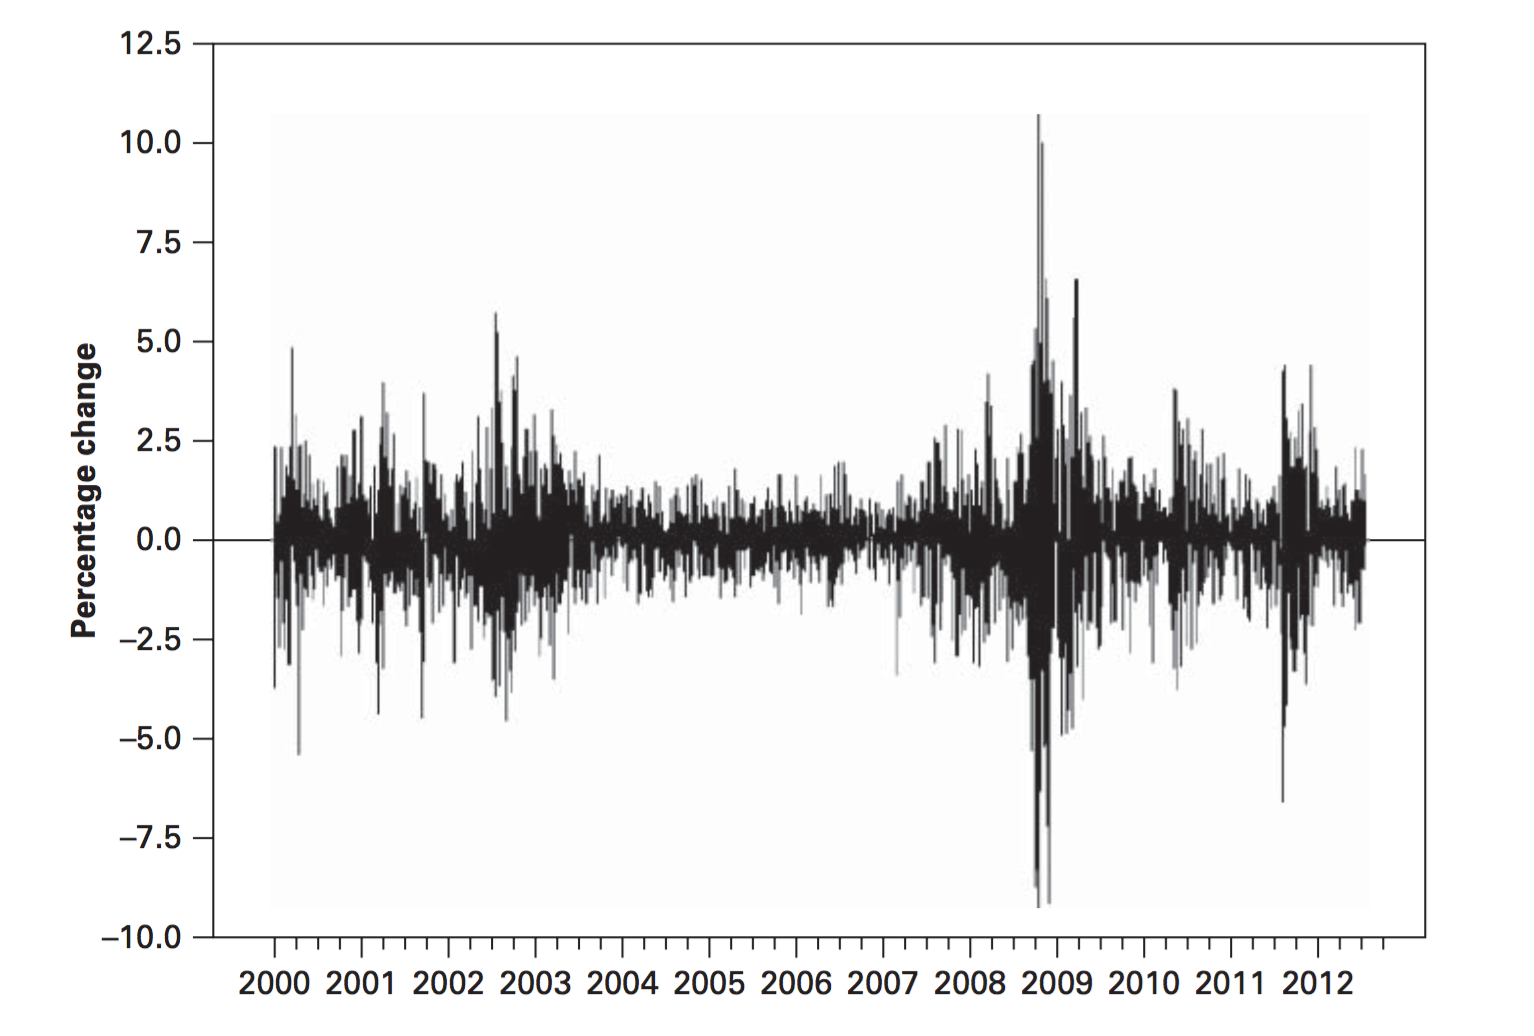
\includegraphics[width=\textwidth]{img/nyse_us100.png}
\caption{\label{fig:orgda0005e}
Percentage Change in the NYSE U.S. 100}
\end{figure}

\item \textbf{Volatility evolves over time in a continuous manner.} That is,
volatility jumps are rare. In Figure \ref{fig:orgcf3aa34}, the change of the
volatility of the annualized real GDP growth rate of the U.S. is
relatively smooth. 

\begin{figure}[htbp]
\centering
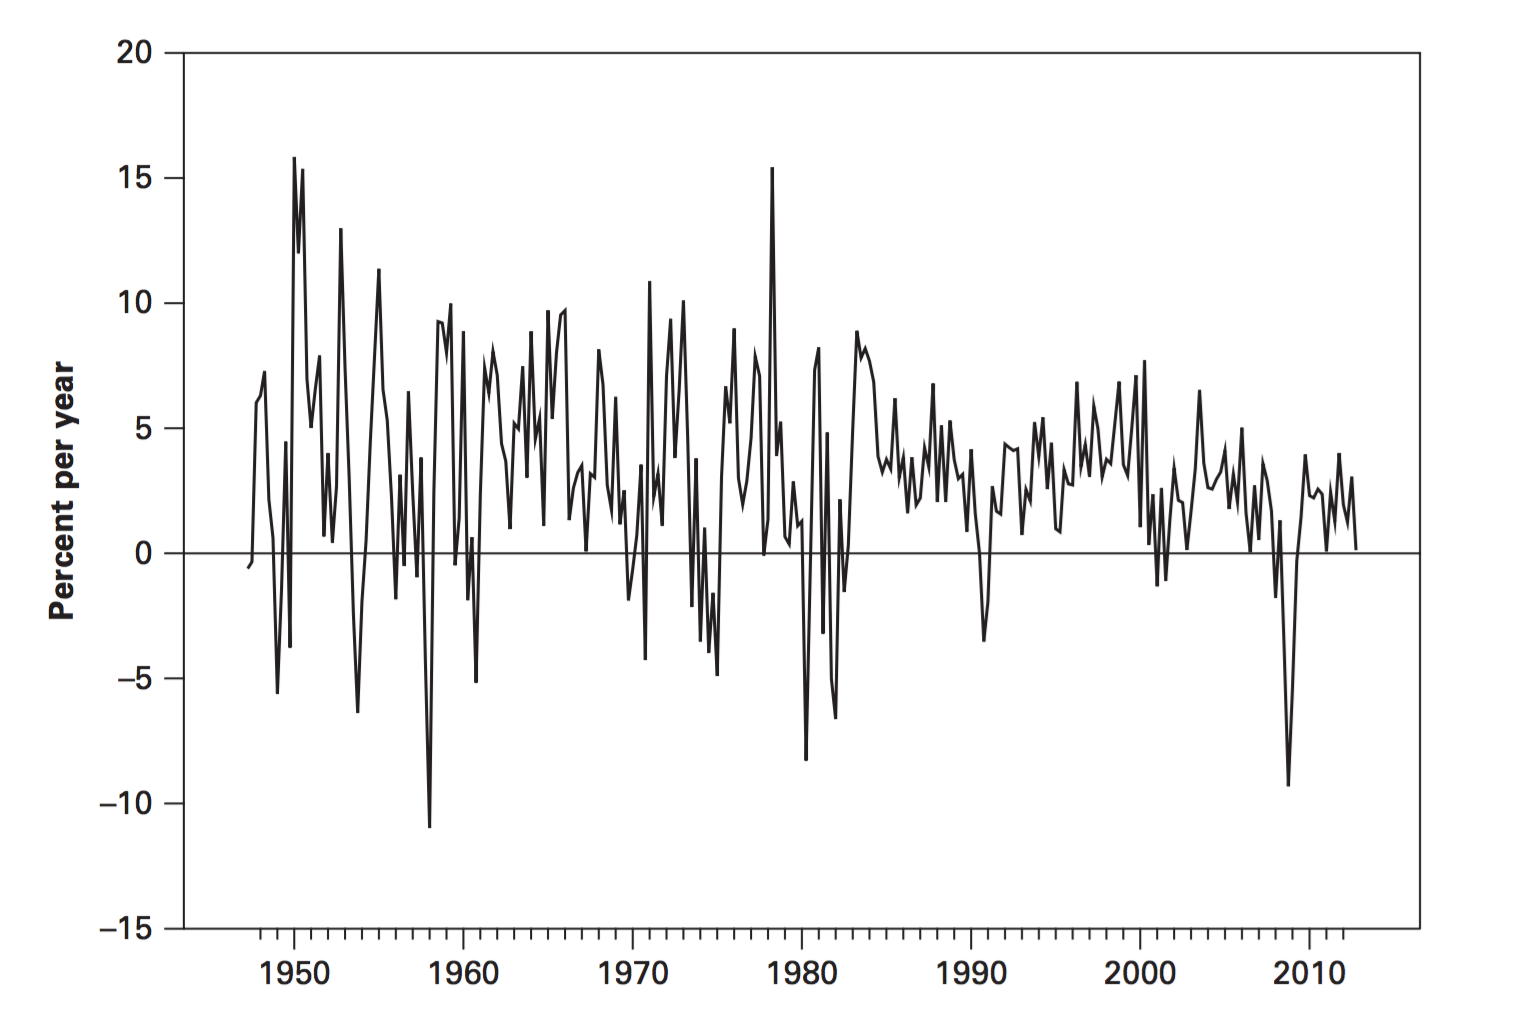
\includegraphics[width=\textwidth]{img/readgdp.png}
\caption{\label{fig:orgcf3aa34}
Annualized Growth Rate of Real GDP}
\end{figure}

\item \textbf{Volatility does not diverge to infinity.} That is, volatility varies
within some fixed range. Statistically speaking, this means that
volatility is often stationary.

\item Volatility seems to react differently to a big price increase or a
big price drop, referred to as \textbf{the leverage effect}.
\end{enumerate}


\section{The Structure of a Volatility Model}
\label{sec:orgef13e99}

\subsection{The basic idea of building a volatility model}
\label{sec:org687c221}

Consider the log return series \{\(r_t\)\}. The basic idea of a volatility
model is that \{\(r_t\)\} may appear to be either serially uncorrelated or
serially correlated with a minor order, but \{\(r_t\)\} is a dependent
series and the dependence arises from its conditional variance. 

\begin{figure}[htbp]
\centering
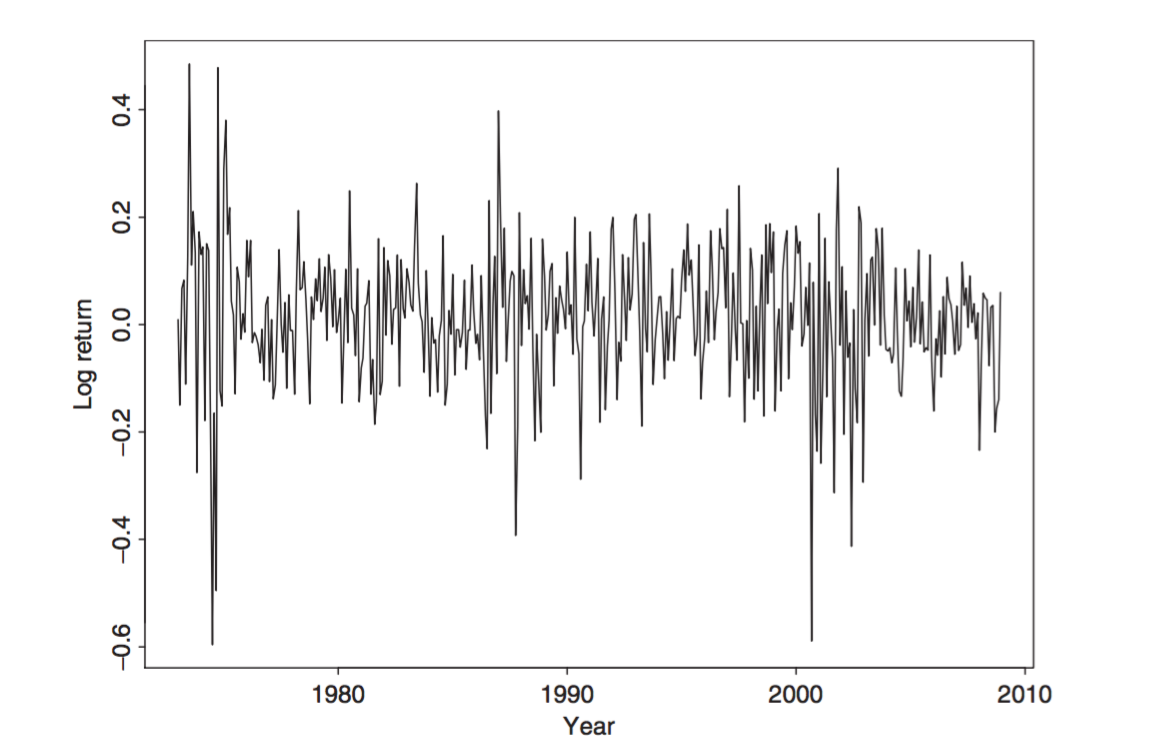
\includegraphics[width=\textwidth]{img/intel.png}
\caption{\label{fig:org2b79565}
Time plot of monthly log returns of Intel stock from January 1973 to December 2008}
\end{figure}

\begin{figure}[htbp]
\centering
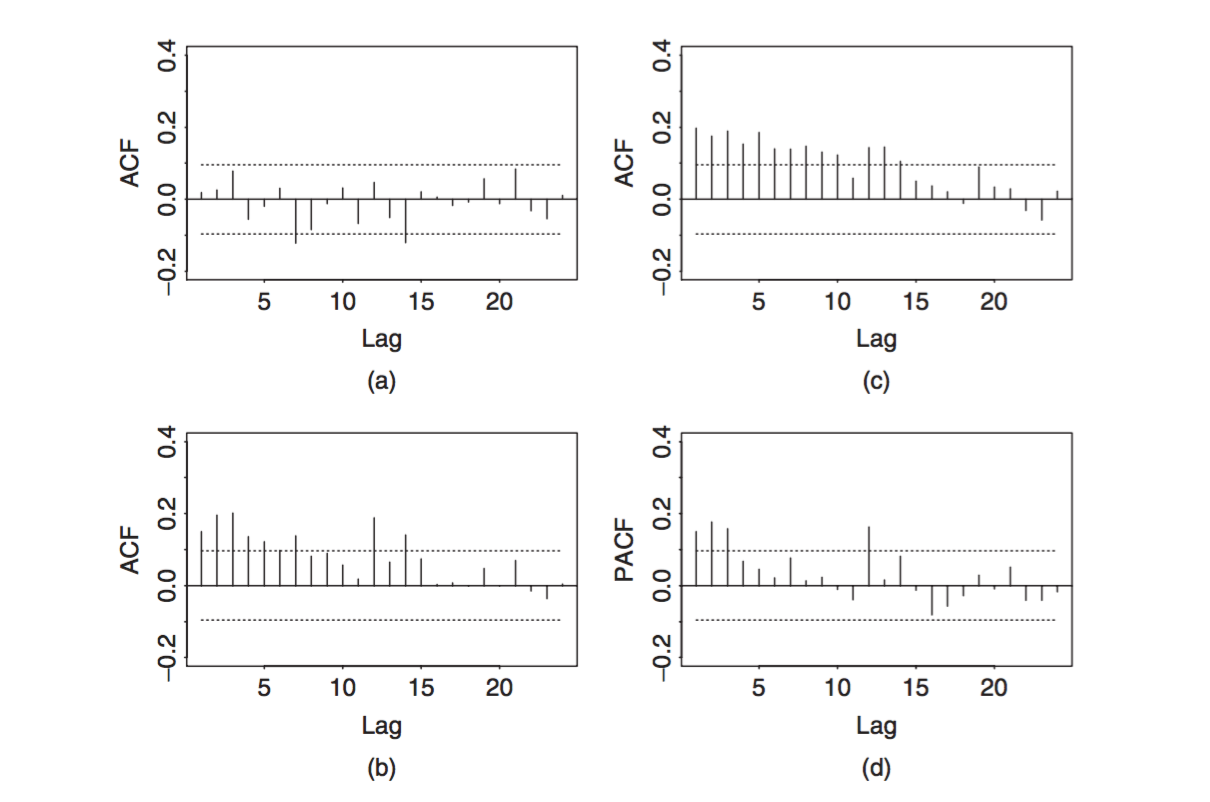
\includegraphics[width=\textwidth]{img/acf_intel.png}
\caption{\label{fig:orgca9e0cf}
Sample ACF and PACF of various functions of monthly log stock returns of Intel Corporation from January 1973 to December 2008: (a) ACF of the log returns, (b) ACF of the squared log returns, (c) ACF of the absolute log returns, and (d) PACF of the squared log returns.}
\end{figure}

For illustration, consider the monthly log stock returns of Intel
Corporation from January 1973 to December 2008 shown in Figure
\ref{fig:org2b79565}. 

Figure \ref{fig:orgca9e0cf} displays the sample ACF and PACF of the
log return. 
\begin{itemize}
\item Figure \ref{fig:orgca9e0cf}(a) shows the sample ACF of the log
return series \{\(r_t\)\}, which suggests no significant serial correlations
except for a minor one at lag 7.
\item Figure \ref{fig:orgca9e0cf}(b) shows the sample ACF of the squared log returns
\{\(r^2_t\)\}, which shows strong autocorrelation in the first few
lags.
\item Figure  \ref{fig:orgca9e0cf}(c) shows the sample ACF of the
absolute log returns, also showing strong autocorrelation.
\end{itemize}

These two plots clearly suggest that the monthly log returns are not
serially independent. Combining the three plots, it seems that the
log returns are indeed serially uncorrelated but
dependent. Volatility models attempt to capture such dependence in
the return series.


\subsection{The mean equation and the volatility equation}
\label{sec:org11942d0}

To capture the dependence in a time series through its second moment
but not the mean, we model the mean process and the variance process
separately. 

For a return series \{\(r_t\)\}, we can model it as
\begin{equation}
\label{eq:mean-plus-var}
r_t = \mu_t + a_t
\end{equation}
where \(\mu_t\) represents the conditional mean and \(a_t\) is
modeled to capture the conditional variance.

\subsubsection*{The mean equation}
\label{sec:org4e9afeb}

The mean equation is essentially an ARMA(p, q) model that is defined in
terms of the conditional mean. 

\begin{align}
&\mu_t = E(r_t \mid F_{t-1}) = \sum_{i=1}^p \phi_i y_{t-i} - \sum_{i=1}^q \theta_i a_{t-i} \label{eq:mean-equation} \\
&y_t = r_t - \phi_0 - \sum_{i=1}^k \beta_i x_{it} \nonumber
\end{align}
\(F_{t-1}\) is the information set at time \(t-1\). If you combine these
two equations, and let \(\mu_t = r_t - a_t\), you will find that it is
just an ARMA\((p, q)\) model with additional regressors \(x_{it}\).

\subsubsection*{The variance equation}
\label{sec:orgb52c959}

Let's see what is the conditional mean of \(r_t\). Denote the
conditional variance of \(r_t\) with \(\sigma^2_t\). 
\begin{equation*}
\begin{split}
\sigma^2_t = \var(r_t \mid F_{t-1}) &= E\left( (r_t - E(r_t | F_{t-1}))^2 | F_{t-1} \right) \\
&= E\left( (r_t - \mu_t)^2 \mid F_{t-1} \right) \\
&= \var(a_t \mid F_{t-1})
\end{split}
\end{equation*}

If we assume that \(E(a_t \mid F_{t-1}) = 0\), we can see that
\(\sigma^2_t = E(a^2_t \mid F_{t-1})\). This result motivates us to use
the series of \{\(a^2_t\)\} to model the conditional variance
\(\sigma^2_t\). The simplest model is a linear model, like the following
\[ \sigma^2_t = \alpha_0 + \alpha_1 a^2_{t-1} + \cdots + \alpha_m a^2_{t-m} \]
Let \(a^2_t = \sigma^2_t + \nu_t\) where \(\nu_t\) is a white noise
series. The above equation turns into an AR\((m)\) model for \{\(a^2_t\)\}
as follows
\[a^2_t = \alpha_0 + \alpha_1 a^2_{t-1} + \cdots + \alpha_m
a^2_{t-m} + \nu_t \]
This equation represents the essential idea of an ARCH model with just
a little modification. 


\subsection{The procedure of building a volatility model}
\label{sec:org18ab44f}

Building a volatility model for an asset return series consists of
four steps:

\begin{enumerate}
\item Specify a mean equation by testing for serial dependence in the
data and, if necessary, building an econometric model (e.g., an
ARMA model) for the return series to remove any linear dependence.

The goal of this step is to get a series of residuals that does not
display any autocorrelation.

\item Use the squared residuals of the mean equation to test for ARCH
effects.

\item Specify a volatility model if ARCH effects are statistically
significant, and perform a joint estimation of the mean and
volatility equations.

\item Check the fitted model carefully and refine it if necessary.
\end{enumerate}


\subsection{Testing for the presence of ARCH effect}
\label{sec:orgd21a16d}

\subsubsection*{The Ljung-Box test for the series of \(a^2_t\)}
\label{sec:org0849fa4}

Upon obtaining the residuals from the estimation
of an adequate mean equation, we can use the squared residuals
\{\(\hat{a}_t^2\)\} to test the existence of autocorrelation. 

The Ljung-Box test is used to test the null hypothesis
\(H_0: \rho_1 = \cdots = \rho_m = 0\). The \(Q(m)\) statistic is
calculated and compared with the critical value from \(\chi^2(m)\)
distribution at the desired significance level. The rejection of the
null hypothesis implies that there is autoregressive conditional
heteroskedastic (ARCH) effect. 

\subsubsection*{The LM test}
\label{sec:org18d7a39}

We estimate a AR\((m)\) model regarding \{\(\hat{a}^2_t\)\}, that is,
\[ \hat{a}^2_t = \alpha_0 + \alpha_1 \hat{a}_{t-1}^2 + \cdots +
\alpha_m \hat{a}^2_{t-m} + e_t \]

With this model, we test the joint hypothesis
\[H_0: \alpha_1 = \cdots = \alpha_m = 0 \]

The LM statistic is \(NR^2\) where \(N\) is the sample size of this
regression and \(R^2\) is the coefficient of the determination of this
regression. Given the null hypothesis is true, this statistic follows
a \(\chi^2(m)\) distribution. 

Alternatively, we can use F statistic to test the joint
hypothesis. 
\begin{itemize}
\item Let \(SSR_0 = \sum_{t=m+1}^{T} (\hat{a}^2_{t} -
  \bar{\omega})^2\), where \(\bar{\omega} = (1/T) \sum_{t=1}^T
  \hat{a}^2_t\). \(SSR_0\) is in fact the restricted sum of squared
residuals from the above regression with the \emph{m} restrictions
\(\alpha_1 = \cdots = \alpha_m = 0\).
\item Let \(SSR_1 = \sum_{t=m+1}^T \hat{e}^2_t\) where \(\hat{e}_t\) is the
residuals from the regression. \(SSR_1\) is the unrestricted SSR. The
degree of freedom of \(SSR_1\) is \(T-2m-1 = (T-m) - (m+1)\).
\item The F statistic is
\[F = \frac{(SSR_0 - SSR_1)/m}{SSR_1/(T-2m-1)} \sim F(m, T-2m-1)\]

When \(T \rightarrow \infty\), we know \(mF\) is asymptotically
distributed as a \(\chi^2(m)\) distribution.

\item Rejecting the null hypothesis motivates us to model the possible
ARCH effect.
\end{itemize}

\subsubsection*{An example}
\label{sec:org2b65c2c}

Go back to Figure \ref{fig:orgca9e0cf}. Since the return series is
already stationary, we directly test the squared return series to
check the ARCH effect. 

In the LM test of the ARCH effect, \(F = 53.62\) and the p value is
close to zero. The Ljung–Box statistics of the \(a^2_t\) series also
shows strong ARCH effects with \(Q(12) = 89.85\), the p value of which is
close to zero. Therefore, we can confirm that the return series of
Intel stock has an ARCH effect, and next we need to model such an
effect. 
\end{document}